#!/usr/bin/python
# -*- coding: utf8 -*-
  
import os, re

print(r"""
\include{layout/header}

% infos über thema, author und uni
\newcommand{\art}{}
\renewcommand{\author}{Steve Göring}

\newcommand{\thema}{CloudTag \\{\small --Ein Tag Cloud Generator-- } \\[2em] {\small Programmierwettbewerb \\ Freies Magazin 04-2012 } }


\begin{document}
    
    % titelseite einfügen
    \begin{titlepage}
   
    \centering
    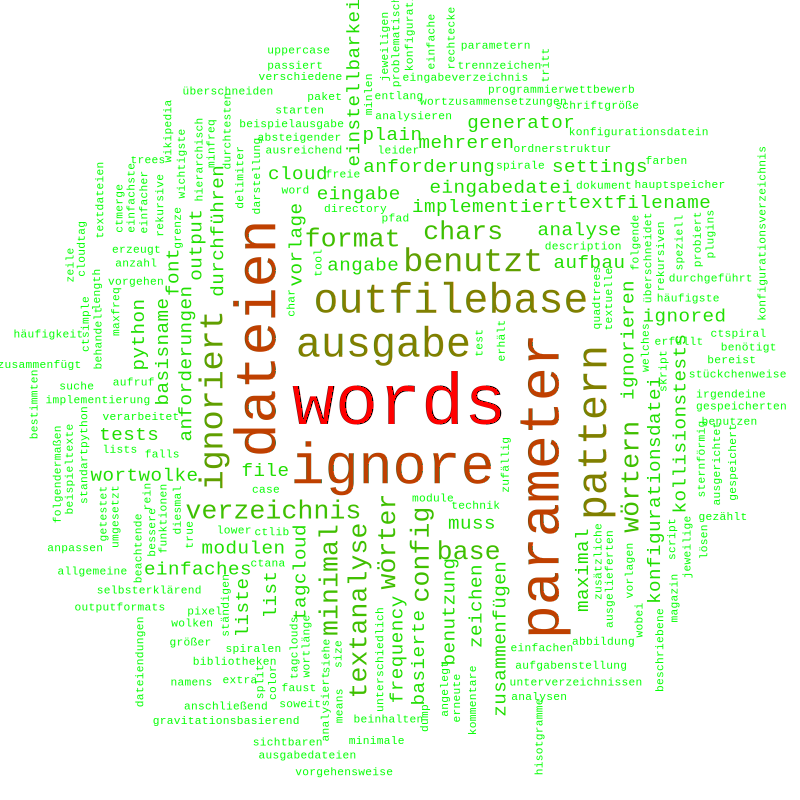
\includegraphics [width=0.9\textwidth] {images/doc.pdf} \\[1em]
    
    
    ~\\[2em]

    % thema
     
    {\LARGE \bf \thema} \\[1cm]
    
    % authoren infos
    \begin{tabular}{rl}
        von:  & \onecm \author \\[0.5em]
        Datum: & \onecm \today \\[0.5em] 
        \hline
    \end{tabular}
    \\[10em]
    
    
\end{titlepage}


\clearpage
 

    
    
    \tableofcontents %\tableofcontents
    
    \newpage
   
    \pagenumbering{arabic}
    % inhalt einfügen
""")

includefiles = []
for f in sorted(os.listdir("content")):
    s = f.split(".")
    if(len(s)==2 and s[1] == "tex"):
        includefiles.append(s[0])

# include all tex files in content directory
for f in includefiles:
    print(r"    \include{content/" + f + "}")
   
print(r"""    


\end{document}
""")


